 
\documentclass[10pt]{article}         %% What type of document you're writing.
\usepackage{graphicx}
\usepackage{hyperref}
\usepackage[dvipsnames]{xcolor}

%%%%% Preamble

%% Packages to use

\usepackage{amsmath,amsfonts,amssymb}   %% AMS mathematics macros

%% Title Information.

\title{Red Neuronal (Simbolos del teclado)}
\author{Jonathan Roman Gomez}
%% \date{2 July 2004}           %% By default, LaTeX uses the current date

%%%%% The Document

\begin{document}

\maketitle

\begin{abstract}
This document implements the neural network for keyboard symbols.
\end{abstract}

\section{Introduccion}

El objetivo de este proyecto es reconocer caracteres de textos mediante una red neuronal. Distinguimos dos fases en el proceso: En la primera crearemos un prototipo de la red neuronal en MATLAB para conseguir el objetivo de reconocer los diferentes simbolos, mientras que en la segunda fase partimos de un codigo del libro de llamado nonlinear Workbook 3ed , el cual es modificado adecuadamente a nuestro proposito. Tambien mostrare mis resultados de la red neuronal.
\\De igual forma hablaremos de la red neuronal sobre el tema de simbolos de teclado, los datos son presentados en matrices de 9 * 9, antes de iniciar con el desarrollo del codigo se realizara un prototico en la herramienta Octave para verificar que se obtendran los resultados esperados cuando se ejecute el programa.

Para realizar el prototipo de la red neuronal en Octave se crearan matrices de 9*9 ya que al multiplicar el resultado es 81 datos que se ocuparan en la formula que nos proporciono el libro antes mencionado se multiplicara N * 0.15 obtenemos la cantidad de simbolos que se reconoceran, es decir, 81 * 0.15 = 12.15 por tanto el resultado es suficiente para los datos.

\begin{figure}[htb]
\centering
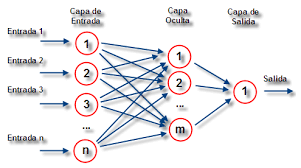
\includegraphics[width=0.5\textwidth]{red neuronal.png}
\caption{Model Neural Network Example}
\label{fig:tigre}
\end{figure}

\section{Desarrollo}
Primero para trabajar en el reconocimiento de patrones debemos encontrar una única estructura de datos que nos permita representar todos los elementos que deseamos reconocer. Para entrenar la red neuronal se debe usar Octave que está desarrollado en MATLAB Para lograrlo, en nuestro caso, hemos seguido los siguientes pasos:
Representar los patrones de la matriz: para representar tanto los símbolos del teclado se usó una matriz de 9*9, para representar un símbolo en dicha matriz, será poner el valor uno (1) en las celdas por donde pasa la marca del número y el valor menos uno (-1) en caso contrario. Por ejemplo, el símbolo se podría representar tal como muestra la figura 2

\begin{figure}[htb]
\centering
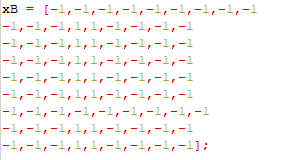
\includegraphics[width=0.5\textwidth]{matriz.png}
\caption{Model Matriz Example}
\label{fig:tigre}
\end{figure}

En el Octave lo que se hara es comprar los valores de entrada y se entregara el valor que mas se parece, dicho eso llamaremos nuestros valores de entrada x,x1,x2,x3 y N, realizaramos la suma de los valores antes mencionados y los guardamos en la variable W despues de esto se haran diferentes calculos para ir comparando cada patron con el mas parecido con el que deseamos que se muestre en consola.

Despues de que se comprobo que funcionara como lo esperado se empezara a crear el codigo de la red neuronal en c++, en este caso la matriz se representara sera poner el valor 1 en las celdas por donde pasa el marca del numero y el valor 0 en caso contrario rellenando una matriz de 9 * 9 como se puede observar en la figura 3.

\begin{figure}[htb]
\centering
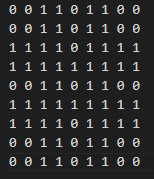
\includegraphics[width=0.2\textwidth]{matriz2.png}
\caption{ejemplo de Matriz}
\label{fig:tigre}
\end{figure}

A continuacion se representa uno de los caracteres que se desea reconocer usando las estructura de datos, representando diversos modelos. aunque aqui solo de mostrara el patron de entrada y el de salida, para realizar el trabajo de reconocerlo entre los demas patrones.

\begin{figure}[htb]
\centering
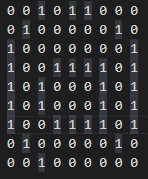
\includegraphics[width=0.3\textwidth]{patron de entrada.png}
\caption{Matriz de entrada a reconocer}
\label{fig:tigre}
\end{figure}

La estructura de datos para representar los datos de salida permitira saber si un elemento de entrada ha sido reconocido o no por nuestra RNA. Por lo tanto, como en nuestro caso solamente deseamos reconocer, en nustro caso nuestro patron de entrada si fue reconocido, se muestra la salida en la siguiente figura 5

\begin{figure}[htb]
\centering
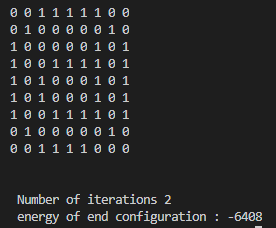
\includegraphics[width=0.4\textwidth]{patron de salida.png}
\caption{Matriz reconocida}
\label{fig:tigre}
\end{figure}
\section{Conclusion}
 Como resultado de este trabajo podemos concluir que el uso de las Redes Neuronales es una gran alternativa para la solucion de muchos probelmas.

Usando como base los resultados mostrados podemos resolver prblemas mas complejos como por ejemplo,reconocimiento de los patrones de la conducta humana, reconocimiento de enfermedades cardiacas, etc.

Debelidad que representa este trabajo es que es una solucion muy basica, pero al mismo tiempo creo que permite apreciar en detalle la entrada y salida sobre el reconocimiento de patrones que es la base de la vision artificial. 

\end{document}